\documentclass[a4paper]{article}
\usepackage[T1]{fontenc}
\usepackage[english]{babel}
\usepackage[utf8]{inputenc}
\usepackage[margin=3cm]{geometry}
% \usepackage{amsmath}
% \usepackage{amssymb}
\usepackage{parskip}
% \usepackage{csquotes}
% \usepackage[hyperref,backend=biber,style=ieee,isbn=true,urldate=iso8601]{biblatex}
\usepackage[colorlinks=true, allcolors=blue]{hyperref}
% \usepackage{listings}
\usepackage{graphicx}

%% Hyperref options
\makeatletter
\hypersetup{
    linktoc=all,
    unicode=true,
    pdfcreator=,
    pdftitle={\@title},
    pdfauthor={\@author},
    pdfdisplaydoctitle=true,
}

\title{Project Mission - EasyTrip}
\author{Jonathan Ahlström \and Ossian Gewert \and Jacob Jönsson \and Simon Persson \and André Roxhage \and Felix Sundholm}

\begin{document}

\maketitle

\begin{center}
    ETSN15 Requirements Engineering

Group Gamma

Jonathan Ahlström
Ossian Gewert
Jacob Jönsson
Simon Persson
André Roxhage
Felix Sundholm  % Group name
\end{center}

\tableofcontents  % auto generated

\section{Background, purpose and goals}
\subsection{Background}
The travel industry is a large and competetive sector with many different actors.
The market is dominated by a few large companies,
which makes it hard for smaller companies to compete.
In the recent years,
services like Momondo and Flight Scanner have gained popularity by offering a service that compares prices from different airlines.
This has made it easier for customers to find the best prices for their flights.
However, these services are not perfect and there is still room for improvement. 

In this project, we will develop a new service called EasyTrip. The goal of EasyTrip is to provice a better service than the existing ones. We will do this by offering a more user-friendly and interactive interface, as well as by providing accurate and up-to-date information. By chosing a starting point, we will compare and visualize flight prices using a map. This will make it easier for the user to find the best prices for their flights, while also exploring new destinations.

\subsection{Purpose}
The purpose of this product is to provide an easy-to-use travel planning tool that enhances customer satisfaction by comparing flight prices efficiently across different geographic areas.

\subsection{Business Goals}
\begin{itemize}
    \item Increase market share by competing with established platforms like Momondo and Flight Scanner.
    \item Generate revenue through partnerships with travel agencies and ad placements.
    \item Build a user base of travelers who trust the platform for accurate price comparisons.
\end{itemize}

\section{Product Context Diagram}
User Roles:
\begin{itemize}
    \item \textbf{Primary Users}: Travelers aged 18-65, using the platform to plan trips.
    \item \textbf{Secondary Users}: Family and friends involved in the traveler’s plans.
    \item \textbf{Tertiary Users}: Travel agencies providing data and bookings.
    \item \textbf{Non-Obvious Actors}: Customer experience support teams ensuring user satisfaction.
\end{itemize}

External Systems:
\begin{itemize}
    \item \textbf{Trip planning Integration}: Retrieve flight price information and availability from travel agencies such as SAS, Norwegian, etc.
    \item\textbf{Map Integration}: Sync with Google Maps for retrieving geographical data, including locations, distances, and travel routes.
\end{itemize}

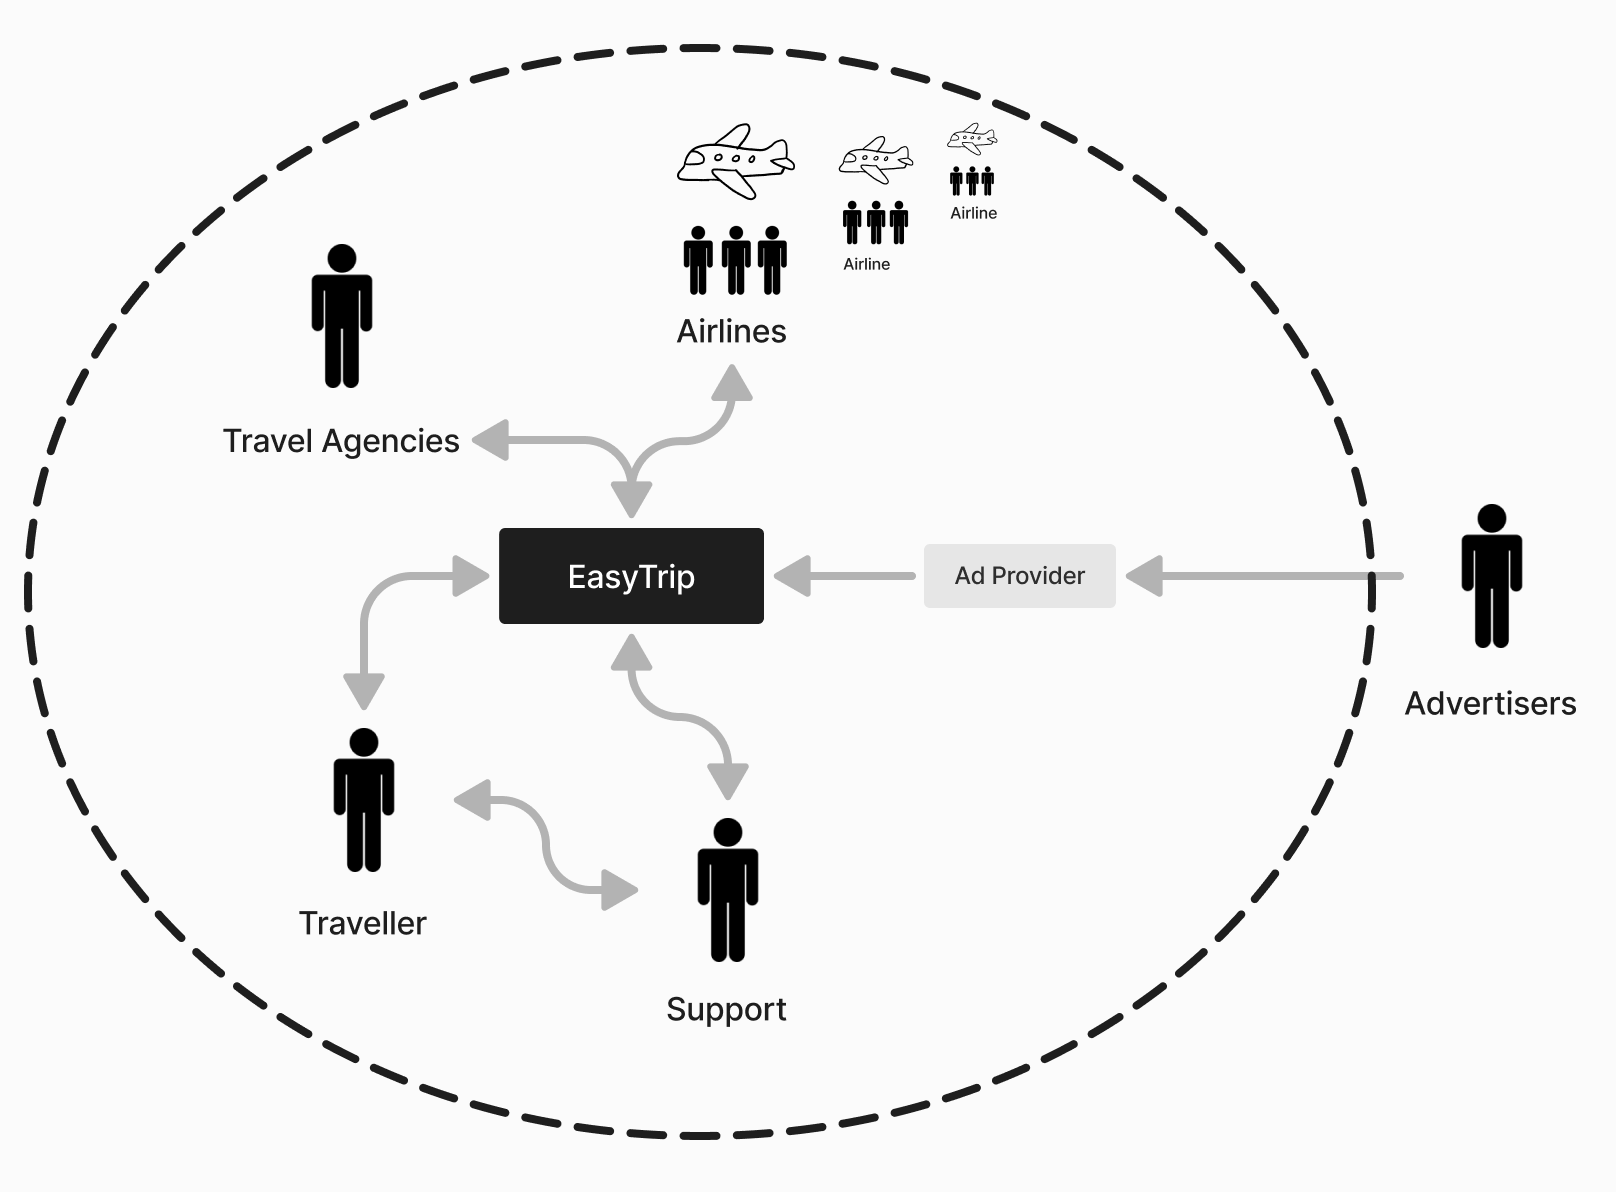
\includegraphics[width=.95\textwidth]{../Release 1/resources/contextDiagram.png}


\section{Participants and Stakeholders}
Jonathan Ahlström, Ossian Gewert, Jacob Jönsson, Simon Persson, André Roxhage and Felix Sundholm.
\subsection{Stakeholders}
\begin{itemize}
    \item Competitors like Momondo and Flight Scanner.
    \item Travel agencies providing data partnerships.
    \item End users (travelers) providing feedback.
    \item Product management and development teams.
    \item Airline companies indirectly benefitting from bookings.
    \item \textbf{Non-obvious Actors}: Support department (Customer Experience)
\end{itemize}


\section{Planned activities}
\subsection{Project Timeline}
\begin{table}[h!]
\centering
\begin{tabular}{|l|l|l|l|l|l|}
\hline
\textbf{Activity}                   & \textbf{Deliverable}         & \textbf{Start Date} & \textbf{End Date} & \textbf{Estimated Hours} & \textbf{Responsible Members}      \\ \hline
Finalize project mission draft      & Project Mission v1           & Jan 20, 2025        & Jan 22, 2025      & 6 hours                  & All team members                  \\ \hline
Revise project mission              & Project Mission v2           & Jan 27, 2025        & Jan 28, 2025      & 6 hours                  & PM, SM, TM                        \\ \hline
Develop first iteration             & Release R1                   & Jan 29, 2025        & Feb 2, 2025       & 14 hours                 & All members                       \\ \hline
Conduct validation planning         & Validation Checklist         & Feb 10, 2025        & Feb 14, 2025      & 5 hours                  & QM, VM                            \\ \hline
Continue development                & Release R2                   & Feb 3, 2025         & Feb 16, 2025      & 19 hours                 & All members                       \\ \hline
Perform validations and report      & Validation Report            & Feb 10, 2025        & Feb 20, 2025      & 10 hours                 & All members, with QM/VM lead      \\ \hline
Final iteration                     & Release R3                   & Feb 17, 2025        & Mar 1, 2025       & 20 hours                 & All members                       \\ \hline
Prepare presentation                & Conference Presentation      & Feb 28, 2025        & Mar 2, 2025       & 5 hours                  & EM, SM                            \\ \hline
Prepare discussant questions        & Discussant Questions         & Mar 1, 2025         & Mar 3, 2025       & 3 hours                  & All members                       \\ \hline
\end{tabular}
\caption{Project Timeline}
\label{tab:project_timeline}
\end{table}

\section{Responsibilities}
\begin{itemize}
    \item \textbf{Project Manager}: Felix Sundholm 
    \item\textbf{Stakeholder Manager}: Ossian Gewert
    \item\textbf{Elicitation Manager}: André Roxhage 
    \item\textbf{Quality Requirements Manager}: Simon Jacobsson Persson
    \item \textbf{Data Reqirements Manager}: Jacob Jönsson
    \item \textbf{Validation Manager}: Jonathan Ahlström
\end{itemize}

\end{document}
